%!TEX root = ../thesis.tex
%*******************************************************************************
%****************************** Second Chapter *********************************
%*******************************************************************************

\chapter{The Rotating Sun}

\section{Differential Rotation}
The sun is known to rotate differentially, unlike the earth. This means that angular rate of rotation of a point in the sun about its spin axis is depends on depth and latitude, $\Omega = \Omega(r,\theta)$. Splitting of p-mode\footnote{pressure waves are also called p-modes} frequencies due to differential rotation is well understood and has a long history of inversion analysis \cite{ritzwoller,lavely92,schou98}.
This $\Omega$ is generally taken to be symmetric about the equitorial plane \cite{ritzwoller}.

As a result of Alfven's freezing theorem\footnote{Alfven's freezing theorem states that in a perfectly conducting plasma, magnetic flux through \textit{every} surface is conserved as it gets dragged along with the ambient flow. See \cite{goedbloed2004} for proof. This theorem implies that magnetic field lines are $frozen$ in the plasma as it flows.}, differential rotation is responsible for winding the solar magnetic field around its spin axis in an axisymmetric fashion. Thus we'll be investigating the effects of an axis symmetric magnetic field on the spectrum in this work, although the method we develop can very well accommodate non-axisymmetric fields too.
\section{Detection from frequency spectrum}
Because of axis symmetry of differential rotation, the flow profile is given as,
\begin{equation}
\vrot = \sum_{s = 1,3,5,...}^{\infty} -w_s^0(r) \partial_{\theta} Y_s^0 \ev{\phi}
\end{equation}

Note that $w_1^0$ is responsible for shell like (pure) rotation as it couples with $\partial_{\theta} Y_1^0 \sim \sin\theta$. Hence $w_3^0$ onwards components of flow are responsible for the differential part of the rotation. The fact that the azimuthal index for the $\vrot$ profile is $0$ means that it has no azimuthal dependence. Finding frequency splittings due to differential rotation is a problem in DPT or QDPT depending on whether we're using the isolated multiplet approximation or not. The isolated multiplet approximation is the assumption that there exists negligible cross coupling between different $\mode{n}{l}$ modes. 
Below we outline the QDPT approach to the problem because when applied to a single multiplet $_n S_l$ it reduces to the DPT approach. It has been argued via analysis differential rotation coupling of \mode{n}{1} and \mode{n}{3} multiplets that eigenfrequency correction to DPT via QDPT from cross coupling between these two is negligible ($\sim 1 \mu Hz$) \cite{lavely92}. We'll show in Chapter 5 (figure \ref{fig:split_dr}) that for $l\sim 100$ modes, a frequency corrections of upto $600 nHz$ frequencies are obtained when QDPT is used.

%which is close to the correction obtained due presence of realistically strong magnetic fields too, and hence cannot be ignored in an analysis which accounts for both differential rotation and magnetic fields.

\subsection{QDPT Analysis}
The pertubation operator \dLd for a differential rotaional flow is given by 
\begin{equation}
\dLd = -2i \omega \rho \vrot \cdot \grad
\end{equation}
where $\omega$ is the reference frequency in the problem, and $\rho$ is the static background density profile \cite{ritzwoller}.
The supermatrix element $Z_{k' k}$ for a pertubation \dLd is given by
\begin{equation}
Z_{k' k} = \Lamdr_{k'k} - \delta_{k'k} (\omref^2 - \omega_k^2)
\end{equation}
where $\Lamdr$ is the coupling matrix element $\Lamdr = \inner{\xiv_{k'}}{\dLd \xiv_{k}}$ .
Coupling matrix element is given by
\begin{equation}
\Lamdr_{k'k} = 8 \pi \omref \gam{l'}\gam{l} \oddsum{s} \gam{s} \wigred{-m}{0}{m} \ints dr 
r^2 w_s^0(r) T_s(r)
\end{equation}
where the sensitivity kernel $T_s$ is given by
\begin{dmath}
T_s(r) = (1-(-1)^{s+l+l'}) \om{l'}{0} \om{l}{0} \wigred{-1}{0}{1} r^{-1}
 \enc{U'V+V'U-U'U-\frac{1}{2}\enc{l'(l'+1) + l(l+1) - s(s+1) V'V}}
\end{dmath}
where the rounded brackets represent Wigner 3j symbols \cite{ritzwoller}, and $\gam{l}$ and $\Omega_{l}^{N}$ are constants defined in Appendix \ref{app_conventions}.
\subsection{Selecition rules in mode coupling}\label{sec:selec_rules}
This matrix element enforces the following selection rules for inter-mode interaction which derive from the properties of Wigner 3j symbols \cite{lavely92}.
\begin{enumerate}
\item $m'=m$
\item $l'+l+s = \text{odd}$
\item $|l'-l| \leq s \leq l'+l$
\end{enumerate}
It should be noted here that even though only sum over odd s is considered, the expression for $T_s$ is general and holds for all $s$. This has been verified independently using the Mathematica packaged developed for the sake of this work \cite{GSH_repo}. Hence, as far as self coupling is concerned ($l'=l$), $T_s$ vanishes for even $s$. This means that even if $\Omega(\theta,\phi)$ had a component which is antisymmetric about the equatorial plane, DPT analysis would not reveal any signature of that in the frequency splittings.

\subsubsection{Form of supermatrix $Z_{k'k}$}

It is clear from selection rule (1) in \ref{sec:selec_rules} that $Z_{k'k}$ is going to be a sparse matrix consisting of a diagonal and a number of sub-diagonals (proportional to number of multiplets being considered). Also, as $s$ is always odd, $l-l'$ has to be even for non-zero coupling as consequence of selection rule (2). This influences our choice of modes whose inter-coupling will be studied hereafter. Figure (\ref{fig:coup_mat}) is a visual representation of a typical supermatrix consisting of three multiplets. The logarithm scale demonstrates the order of magnitude difference between self-coupling (main diagonal elements), and cross-coupling (subdiagonal elements). Also notice that largest elements (yellow) are in the first and third section in the main diagonal. These are large because these frequencies are placed away from $\omref$ which is taken to be mean of the three mode frequencies. The relative weakness of the sub-diagonal terms compared to the main-diagonals is because $l-l'\geq 2$ forces $s\geq 2$ which makes the largest component of differential rotation, i.e. $w_1^0$, unable to couple these modes; $w_3^0$ and $w_5^0$ are one and two orders of magnitude smaller than $w_1^0$ respectively.

\begin{figure}[h]
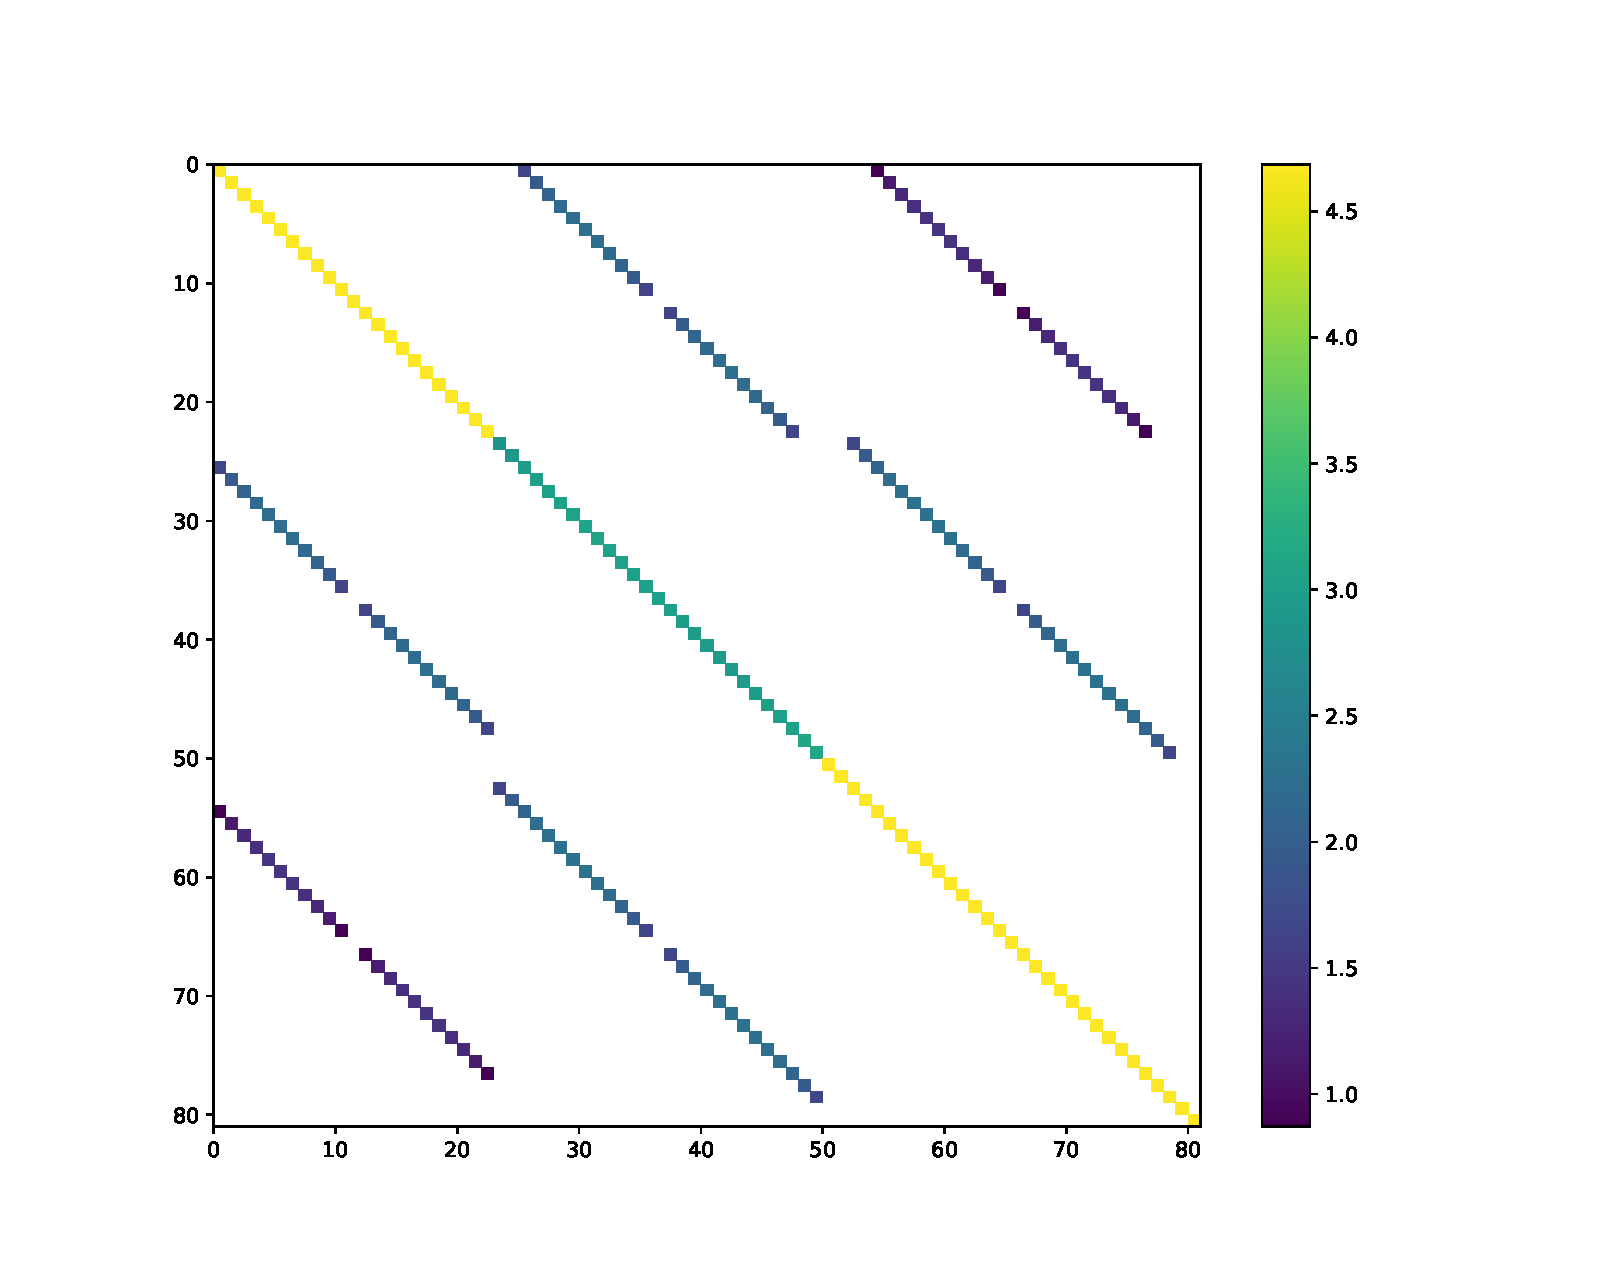
\includegraphics[scale=0.6,center]{Chapter2/figs/coup_mat}
\caption{Visualisation of $\log_{10}|Z_{k'k}|$ in $\mu Hz^2$ for the multiplets $\mode{0}{11}$, $\mode{0}{13}$, and $\mode{0}{15}$ with frequencies $603.69 \mu Hz$, $641.84\mu Hz$, and $677.55 \mu Hz$ respectively. Numbers on the X and Y axes represent cumulative $m$ of all three multiplets. White spaces correspond to $0$ value.}  
\label{fig:coup_mat}
\end{figure}